% Adjust these for the path of the theme and its graphics, relative to this file
%\usepackage{beamerthemeFalmouthGamesAcademy}
\usepackage{../../beamerthemeFalmouthGamesAcademy}
\usepackage{multimedia}
\graphicspath{ {../../} }

\usepackage{textcomp}

% Default language for code listings
\lstset{language=Python, upquote=true,
        morekeywords={each,in,nullptr}
}

% For strikethrough effect
\usepackage[normalem]{ulem}
\usepackage{wasysym}

\usepackage{pdfpages}

% http://www.texample.net/tikz/examples/state-machine/
\usetikzlibrary{arrows,automata}

\newcommand{\modulecode}{COMP260}\newcommand{\moduletitle}{Distributed Systems}\newcommand{\sessionnumber}{5}

\setbeamertemplate{navigation symbols}{}

\newcommand{\fullbleed}[1]{
\begin{frame}[plain]
	\begin{tikzpicture}[remember picture, overlay]
		\node[at=(current page.center)] {
			\includegraphics[width=\paperwidth]{#1}
		};
	\end{tikzpicture}
\end{frame}
}

\newcommand{\picturepage}[2]{
\begin{frame}[plain]
	\begin{tikzpicture}[remember picture, overlay]
		\node[at=(current page.center)] {
			\includegraphics[width=\paperwidth]{#1}
		};
		\draw<1>[draw=none, fill=black, opacity=0.9] (-1,-5.2) rectangle (current page.south east);
		\node[draw=none,text width=0.96\paperwidth, align=right] at (5.5,-5.5) {\tiny{#2}};
	\end{tikzpicture}
\end{frame}
}

\newcommand{\notepicx}[5]{
\begin{frame}[plain]
	\begin{tikzpicture}[remember picture, overlay]
		\node[at=(current page.center)] {
			\includegraphics[width=\paperwidth]{#1}
		};
		\node[draw=none, fill=black, text width=#5\paperwidth] at ([xshift=#3, yshift=#4] current page.center) {\small{#2}};
	\end{tikzpicture}
\end{frame}
}

\newcommand{\notepic}[4]{
	\notepicx{#1}{#2}{#3}{#4}{0.4}
}

\begin{document}
\title{\sessionnumber: Tinkering in Python}
\subtitle{\modulecode: \moduletitle}

\frame{\titlepage} 

\begin{frame}
	\frametitle{Learning Outcomes}
	\begin{itemize}
		\item \textbf{Outline} the role and basic functions of the IDE
		\item\textbf{Interpret} some basic Python code
		\item \textbf{Apply} pair programming practices to solve a simple text concatenation problem
		\item \textbf{Explain how} pictures are digitised into raster images by a computer system
	\end{itemize}
\end{frame}

\part{The PyCharm IDE}
\frame{\partpage}

\begin{frame}{Integrated Development Environment (IDE)}
\begin{itemize}
	\pause\item You \textit{could} just write code in Notepad, but...
	\pause\item An \textbf{Integrated Development Environment (IDE)} is an application providing several
	useful features for programmers, including:
	\begin{itemize}
		\pause\item A ``run'' button
		\pause\item Management of multi-file projects
		\pause\item Syntax highlighting
		\pause\item Autocompletion
		\pause\item Navigation
		\pause\item Language and API documentation
		\pause\item Debugging
		\pause\item Profiling
		\pause\item Version control
	\end{itemize}
\end{itemize}
\end{frame}

\begin{frame}{Setting up your own PC}
\begin{itemize}
\pause\item Python 2.7
\begin{itemize}
	\pause\item \url{https://www.python.org/}
	\pause\item Python 2.7 is included with Mac OSX and most Linux distributions, but needs to be installed separately on Windows
	\pause\item Python 2.x and Python 3.x are (slightly) different programming languages; we are using 2.x (for now)
\end{itemize}
\pause\item PyCharm
\begin{itemize}
	\pause\item \url{https://www.jetbrains.com/student/}
	\pause\item Register with your \texttt{falmouth.ac.uk} email address to obtain PyCharm Professional Edition for free
	\pause\item Runs on Windows, Mac and Linux
	\pause\item Other Python IDEs are available
\end{itemize}
\end{itemize}
\end{frame}

\begin{frame}{PyCharm in the Lab}
	\begin{itemize}
		\pause\item You have to license your account to use PyCharm
		\pause\item Run PyCharm and select \textbf{License server}
		\pause\item In the \textbf{License server address} enter the following \textbf{http://trlicefal.fal.ac.uk}
		\pause\item This will be added to your user profile and you will not need to do this again
	\end{itemize} 
\end{frame}

\begin{frame}{Getting started with PyCharm}
\begin{itemize}
\pause\item Create a new project (from the start-up wizard or from the File menu)
\pause\item We want a ``Pure Python'' project
\pause\item Right-click the project in the panel on the left, and choose ``New $\to$ Python File''
\pause\item Write some code!
\pause\item First run: click ``Run $\to$ Run...'' and choose the Python file
\pause\item Subsequent runs: click the $\blacktriangleright$ button
\end{itemize}
\end{frame}


\newcommand{\socrative}{
	\begin{center}
		Socrative room code: \texttt{FALCOMPED}
	\end{center}
}

\newcommand{\codeslide}[2]{
	\begin{columns}
		\begin{column}{0.48\textwidth}
			\lstinputlisting{#1}
		\end{column}
		\pause
		\begin{column}{0.48\textwidth}
			\begin{center}
				\begin{tabular}{|c|c|}
					\hline
					\textbf{Variable} & \textbf{Value} \\\hline
					#2
				\end{tabular}
			\end{center}
		\end{column}
	\end{columns}
}

\newcommand{\trow}[1]{ & \\ \texttt{#1} & \\ & \\\hline}

\part{Basic Python programs}
\frame{\partpage}

\begin{frame}[fragile]{Your first Python program}
	\begin{lstlisting}
print "Hello, world!"
	\end{lstlisting}
\end{frame}

\begin{frame}[fragile]{Your second Python program}
	\begin{lstlisting}
print "This is a very long line of code which had to be split to fit on the slide, but you should type it as a single line."
print "This is the second line of code."
	\end{lstlisting}
\end{frame}

\begin{frame}[fragile]{Assigning to variables}
	\codeslide{assign0.py}{\trow{a}}
\end{frame}

\begin{frame}{Remember!}
	\begin{itemize}
		\pause\item A program is a \textbf{sequence of instructions}
		\pause\item The Python interpreter executes the \textbf{first line} of your program, then the \textbf{second line},
			and so on
		\pause\item When it reaches the end of the file, it \textbf{stops}
	\end{itemize}
\end{frame}

\begin{frame}[fragile]{Reassigning variables (1)}
	\socrative
	\codeslide{assign1.py}{\trow{a}\trow{b}}
\end{frame}

\begin{frame}[fragile]{Reassigning variables (2)}
	\socrative
	\codeslide{assign2.py}{\trow{a}\trow{b}}
\end{frame}

\begin{frame}[fragile]{Reassigning variables (3)}
	\socrative
	\codeslide{assign3.py}{\trow{big}\trow{small}}
\end{frame}

\begin{frame}[fragile]{Reassigning variables (4)}
	\socrative
	\codeslide{assign4.py}{\trow{a}\trow{b}}
\end{frame}

\begin{frame}[fragile]{Reassigning variables (5)}
	\socrative
	\codeslide{assign5.py}{\trow{a}\trow{b}\trow{c}}
\end{frame}

% / Assignment
% Conditional
% For loop
% While loop
% While 1
% Show PyCharm bouncing ball example -- think about this between now and Michael's session next Wednesday


\part{PASS Challenge}
\frame{\partpage}

\begin{frame}
	\frametitle{PASS Challenge}
	
	Review the WAVE and PyGame mixer modules at:
	
	\url{https://docs.python.org/3.6/library/wave.html}
	
	\vspace{1em}
	
	\url{https://www.pygame.org/docs/ref/mixer.html}
\end{frame}	
	
\begin{frame}	
	\frametitle{PASS Challenge}
	\begin{itemize}
		\item In pairs
		\item \textbf{Implement} audio i/o in Python
		\item \textbf{Read} a wave file as a wave\_read object
		\item \textbf{Play} audio in PyGame using the PyGame Mixer
		\item \textbf{Write} a new wave file as a wave\_write object
	\end{itemize}
	
	You can learn more about audio:
	
	\vspace{1em}
	
	 \url{https://inventwithpython.com/chapter19.html}
	
\end{frame}

\part{Tinkering Graphics}
\frame{\partpage}

\begin{frame}
	\frametitle{Light Perception}
	\begin{itemize}
		\item Colour is continuous:
		\begin{itemize}
			\item Visible light is in the wavelengths between 370nm and 730nm
			\item i.e., 0.00000037 --- 0.00000073 meters
		\end{itemize}
		\item However, we \textit{perceive} light around three particular peaks:
		\begin{itemize}
			\item Blue peaks around 425nm
			\item Green peaks around 550nm
			\item Red peaks around 560nm
		\end{itemize}
	\end{itemize}
\end{frame}

\begin{frame}
	\frametitle{Light Perception}
	\begin{itemize}
		\item Our eyes have three types of colour-sensitive photoreceptor cells called `cones' that respond to light wavelengths
		\item Our perception of colour is based on how much of each kind of sensor is responding
		\item An implication of this is perception overlap: we see two kinds of `orange' --- one that's spectral and one that's combinatorial
	\end{itemize}
\end{frame}

\fullbleed{1416_Color_Sensitivity}

\begin{frame}
	\frametitle{Luminance vs Colour}
	\begin{itemize}
		\item Our eyes have another type of photoreceptor cells called `rods' that respond to light intensity
		\item Our perception, however, is actually luminance: a relativistic contrast of \textit{borders} of things (i.e., motion) 
		\begin{itemize}
			\item Luminance is \textit{not} the amount of light, but our perception of the amount of light
			\item Much of our luminance perception is based on comparison to background, not raw values
		\end{itemize}
		\item An implication of this is perception overlap: we see blue as `darker' than red when the intensity is actually the same
	\end{itemize}
\end{frame}

\fullbleed{grayscale}

\begin{frame}
	\frametitle{Resolution}
	\begin{itemize}
		\item We have a limited number of rods and cones in our eyes
		\item This means humans perceive vision in a limited resolution --- yet, we perceive vision as continuous
		\item We take advantage of this human characteristic in computer monitors
	\end{itemize}
\end{frame}

\fullbleed{sony-dsc-29-625x1000}

\begin{frame}
	\frametitle{Pixels}
	\begin{itemize}
		\item We digitize pictures into many little dots
		\item Enough dots and it looks like a continuous whole to our eye
		\item Each element is referred to as a \textit{pixel}
	\end{itemize}
\end{frame}

\begin{frame}
	\frametitle{Pixels}
	
	Pixels must have:
	
	\begin{itemize}
		\item a color
		\item a position
	\end{itemize}
\end{frame}

\begin{frame}
	\frametitle{Pictures and Surfaces}
	
	In PyGame, a \texttt{Surface} is a \textit{matrix} of pixels
	
	\begin{itemize}
		\item It is not a continuous line of elements, that is, a one-dimensional \textit{array}
		\item A picture has two dimensions: width and height
		\item It's a two-dimensional \textit{array}
	\end{itemize}
\end{frame}

%\fullbleed{pic_array}

%\fullbleed{pic_matrix}

\begin{frame}
	\frametitle{Pictures and Surfaces}
	
	\begin{itemize}
		\item (x, y) ---or--- (horizontal, vertical)
		\item The origin (0,0) is top-left
		\item (1,0) = 12
		\item (0, 2) = 6
	\end{itemize}
\end{frame}

\begin{frame}
	\frametitle{Encoding Colour}
	
	\begin{itemize}
		\item Each element in the matrix is a pixel, with the matrix defining its position and the value defining  its colour
		\item Computer memory stores numbers, so colour must be encoded into a number:
		\begin{itemize}
			\item CMYK = cyan, magenta, yellow, black
			\item HSB = hue, saturation, brightness
			\item RGBA = red, green, blue, alpha (transparency)
		\end{itemize}
		\item By default, Visual Studio and C\# uses RGBA
	\end{itemize}
\end{frame}

\begin{frame}[fragile]
	\frametitle{Encoding RGB}
	
	\begin{itemize}
		\item Each component color (red, green, and blue) is encoded as a single byte
		\item Colors go from %\lstinline{(0,0,0)} to \lstinline{(255,255,255)}:
		\begin{itemize}
			\item If all three components are the same, the colour is in grey-scale
			\item  \lstinline{(0,0,0)} is black
			\item  \lstinline{(255, 255, 255)} is white
		\end{itemize}
	\end{itemize}
\end{frame}



\begin{frame}
	\frametitle{Encoding Bits}
	
	Why \texttt{255}?
	
	\begin{itemize}
		\item If we have one bit, we can represent \textbf{TWO} patterns:
		\begin{itemize}
			\item 0
			\item 1
		\end{itemize}
		
		\item If we have two bits, we can represent \textbf{FOUR} patterns:
		\begin{itemize}
			\item 00
			\item 01
			\item 10
			\item 11
		\end{itemize}
		\item With \textit{n} bits, we can have $2^n$ patterns
		\item With $8$ bits, there will be $256$ patterns
		\item One of these patterns will be $0$, so the highest value we can represent with $8$ bits is: $2^8 - 1$, or $255$
	\end{itemize}
\end{frame}
\begin{frame}
	\begin{center}
		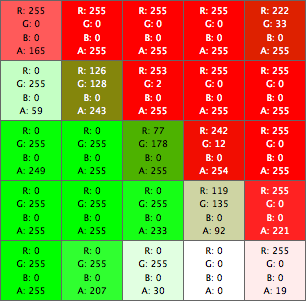
\includegraphics[scale=0.5]{rgb_pallette}
	\end{center}	
\end{frame}
\begin{frame}
	\frametitle{Encoding Bits}
	\begin{itemize}
		\item RGB uses 24-bit color (i.e., $3 * 8$ = 24)
		\begin{itemize}
			\item That's 16,777,216 possible colours
			\item Our eyes cannot discern many colours beyond this
			\item A challenge is display technology: monitors and projectors can`t reliably reproduce 16 million colours
		\end{itemize}
		\item RGBA uses 32-bit colour
		\begin{itemize}
			\item No additional colour, but offers support for transparency
			\item This transparency channel is called \texttt{alpha}
			\item The alpha channel also requires 8 bits
		\end{itemize}
		\item Assuming \texttt{1 byte} == \texttt{8 bits}
		\item We can use this information to estimate the size of a bitmap:
		\begin{itemize}
			\item 320x240x24 = 230,400 bytes
			\item 640x480x32 = 1,228,800 bytes
			\item 1024x768x32 = 3,145,728 bytes
		\end{itemize}
	\end{itemize}
\end{frame}

\fullbleed{texture-254576_1920}

\begin{frame}[fragile]
	\frametitle{Manipulating Bitmap Pixels}
	
	\begin{itemize}
		\item Images are controlled and manipulated using the \texttt{Bitmap} class in C\#
		\item We can use \texttt{GetPixel} and \texttt{SetPixel} methods to both find and change pixels.
	    \begin{lstlisting}
myImage.GetPixel(x, y);
myImage.SetPixel(x, y, newColor);
	    \end{lstlisting}
	    \item Both methods use cartesian coordinates (x and y) to define the position of a specific pixel
	\end{itemize}
\end{frame}

\begin{frame}[fragile]
	\frametitle{Manipulating Bitmap Pixels}
\begin{center}
	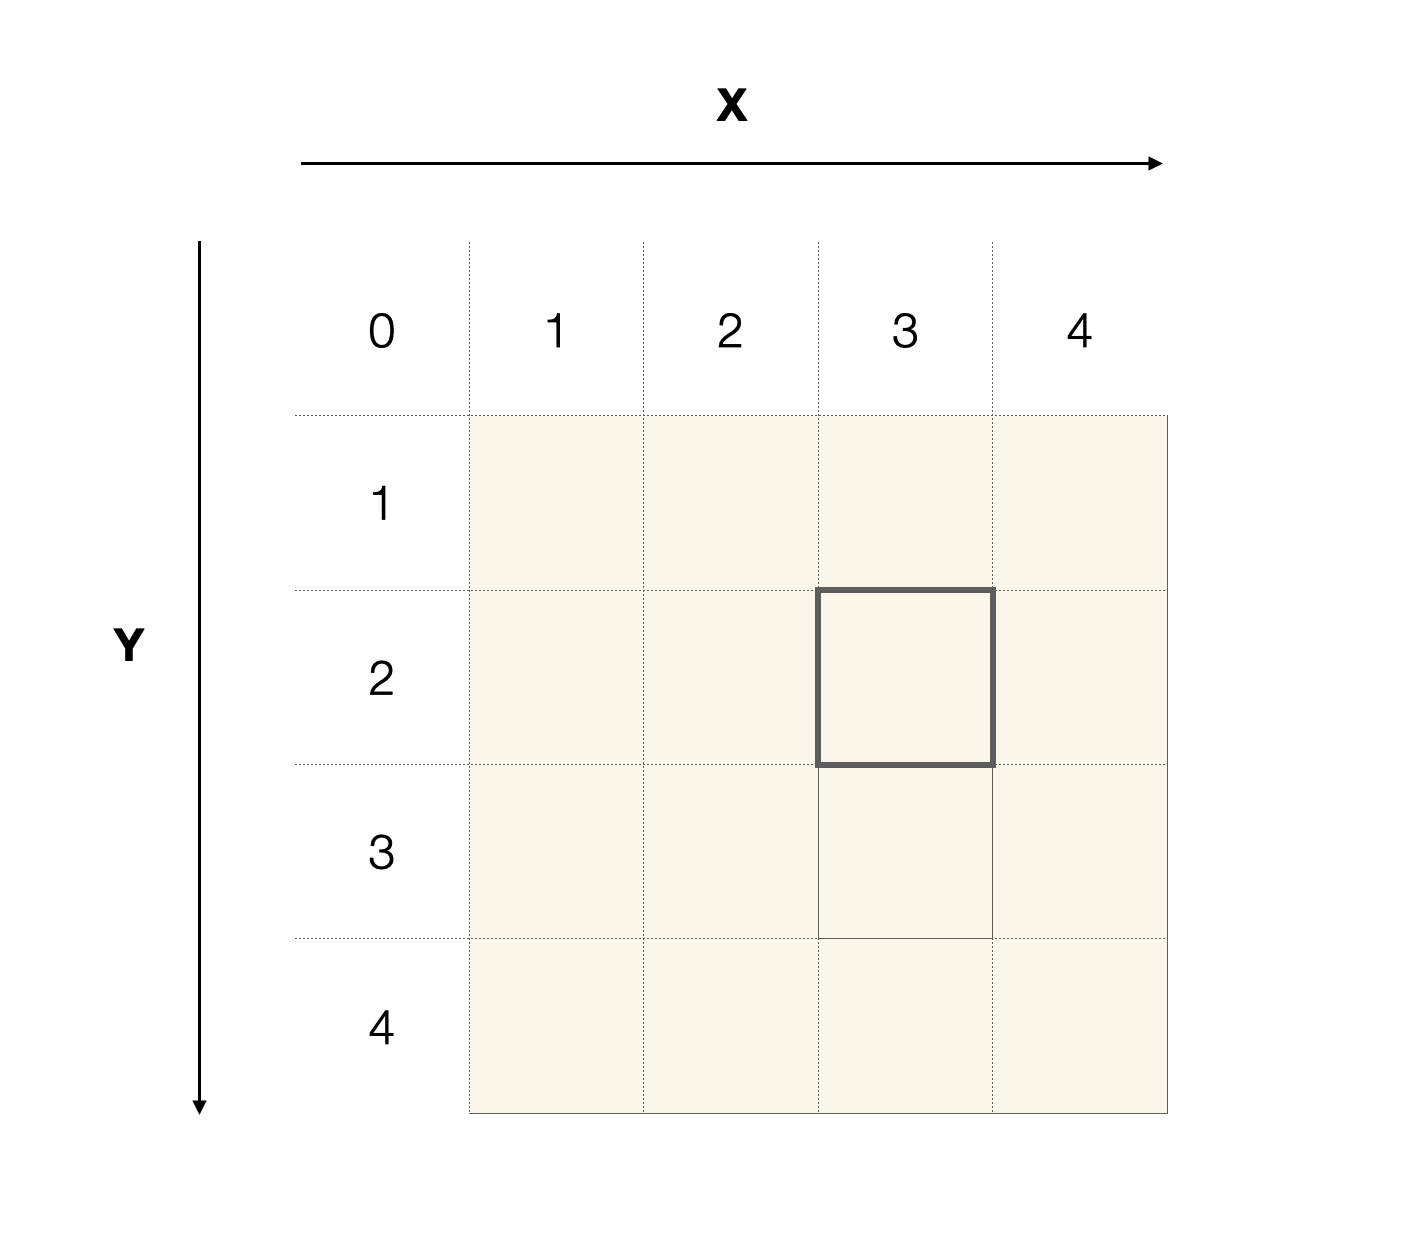
\includegraphics[scale=0.2]{pixel_coordinates}	
\end{center}
	\begin{lstlisting}
myImage.GetPixel(3, 2);
	\end{lstlisting}
	We can use the method to discover the ARGB values at the above position

\end{frame}

\end{document}